%%%%%%%%%%%%%%%%%%%%%%%%%%%%%%%%%%%%%%%%%%%%%%%%%%%%%%%
% Section
%%%%%%%%%%%%%%%%%%%%%%%%%%%%%%%%%%%%%%%%%%%%%%%%%%%%%%%
\section{Example: Billiard Table with 16 Billiard Balls}\label{sec:Examples}

The billiard table in Fig.~\ref{fig:billiardTable} has 16 billiard balls.
The material constants are shown in Table~\ref{table:billiardTableMaterials}.
The cue ball has an initial velocity pointing to the right and hits the the center of the rack (15 other balls) exactly after a short time interval. This results in a symmetric evolution of the balls, as one would expect.
All previously described effects (sliding, rolling, colliding) act together. The hybrid DAE system has $\dim(\bvec{x}) = 13 \cdot 16 = 208$ and there are
about $200$ possible collision pairs. Simulation on a standard PC needs about \SI{20}{\minute} for \SI{5}{\second} of simulation time. 
At the moment, the Modia3D code is implemented for functionality and not tuned for efficiency, so a speed-up is expected in the future.


\begin{figure}[h]
	\centering
	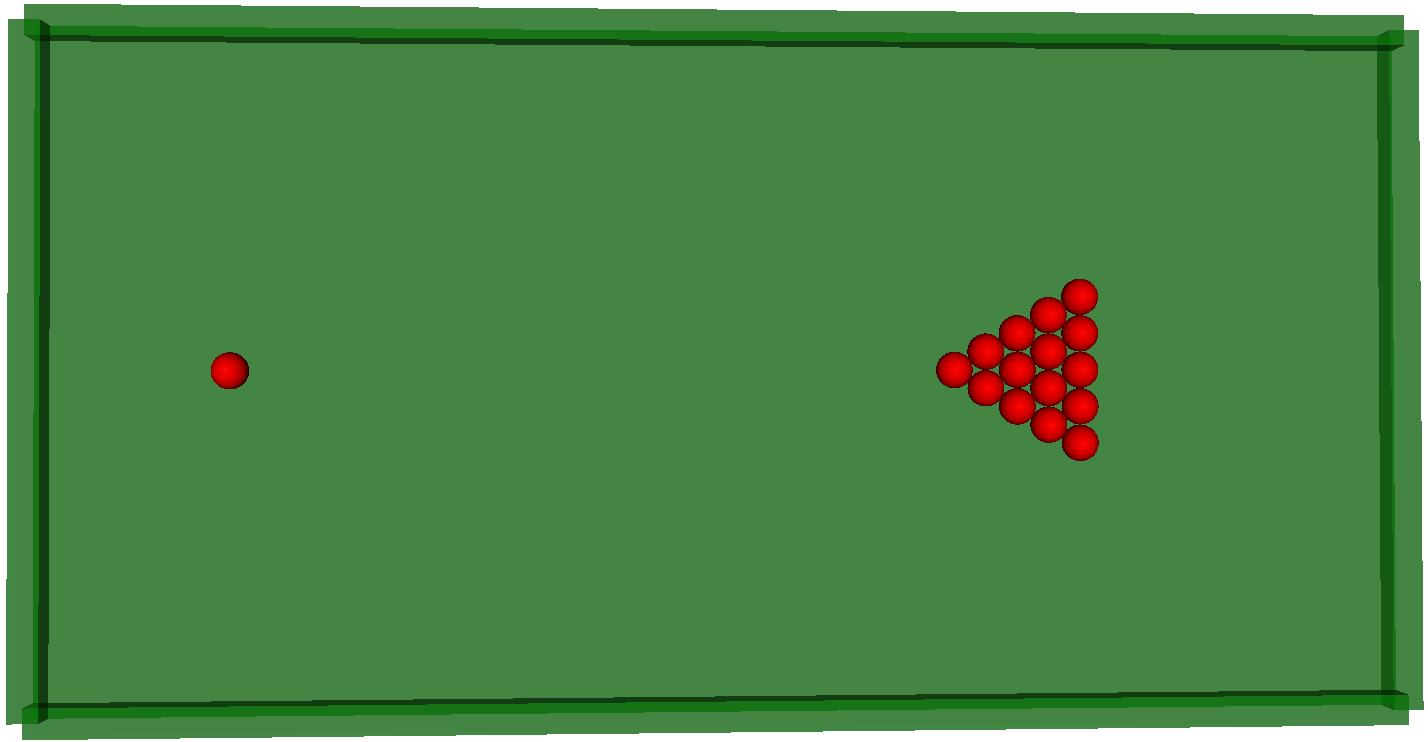
\includegraphics[width=0.35\textwidth]{figures/billiardTableInitial.png}
    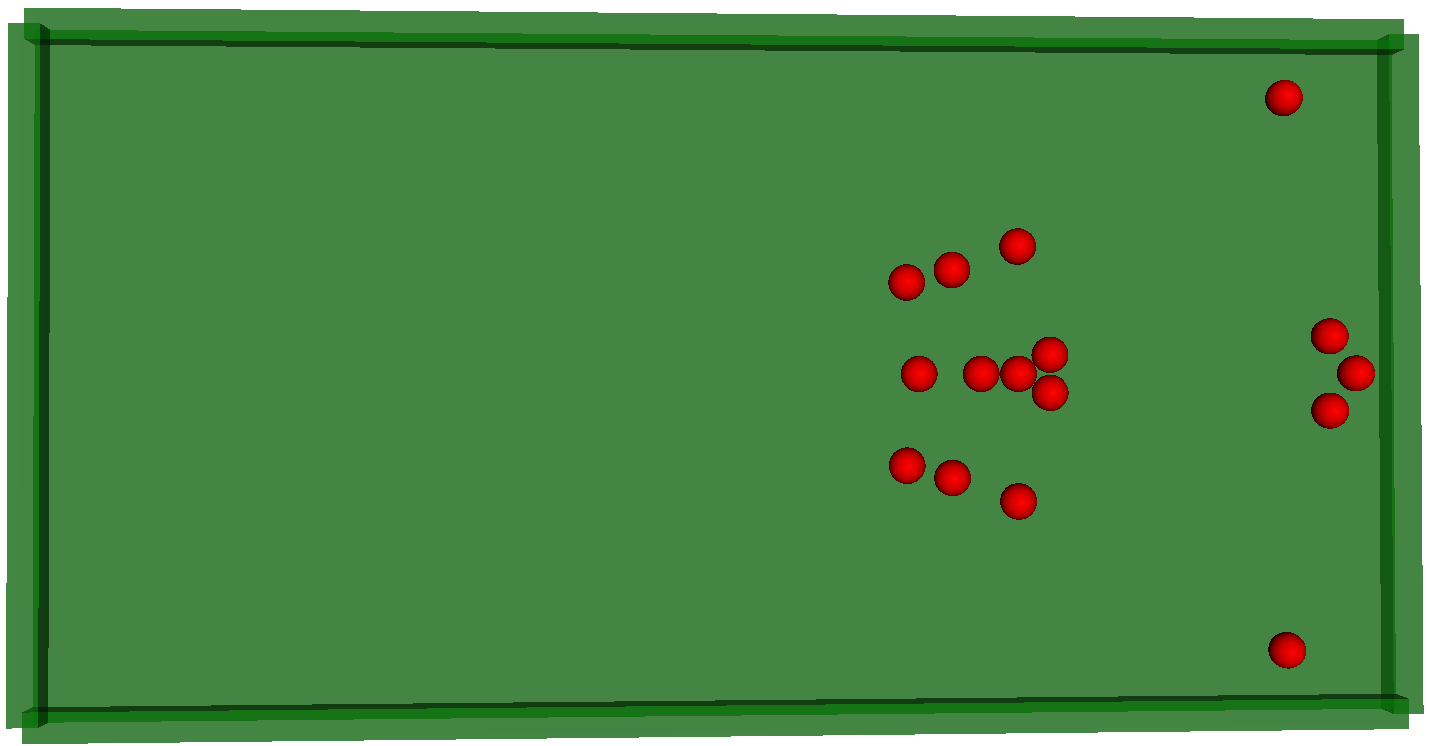
\includegraphics[width=0.35\textwidth]{figures/billiardTable.png}
	\caption{Initial setting of $16$ billiard balls (top). Billiard balls after \SI{5}{\second} (bottom).}
	\label{fig:billiardTable}
\end{figure}
\begin{table}[h]
	\begin{center}
		\tbl{Material constants for billiard table.}{
			\begin{tabular}{llccc}
				\toprule
				&&&    $E$ [$\text{N/m}^2$]   &  $\nu$    \\ 
				\midrule 
				ball        &   &  & $5.4e9$   &  $0.34$    \\ \addlinespace
				table 		&   &  & $1.1e10$   &  $0.4$  \\ \addlinespace
				\midrule
				& & 				 $cor$ & $\mu_k$ & $\mu_r$ \\
				\midrule
				ball   &   table    & 0.0  & 0.6  & 0.02  \\ \addlinespace
				ball   &   ball     & 1.0  & 0.0  & 0.0   \\ \addlinespace
				ball   &   cushion  & 0.8  & 0.0  & 0.0   \\ \addlinespace
		\end{tabular}}  
\label{table:billiardTableMaterials} 
	\end{center}
\end{table}
%











